\documentclass[12pt,a4paper]{article}

% --- KHAI BÁO CÁC GÓI CẦN THIẾT ---
\usepackage{iftex}
\ifXeTeX
  \usepackage{fontspec}
  \setmainfont{Times New Roman}
\else
  \usepackage[utf8]{inputenc}
\fi
\usepackage[vietnamese]{babel} % Hỗ trợ tiếng Việt
\usepackage{geometry}
\geometry{
    a4paper,
    total={170mm,257mm},
    left=30mm,
    right=20mm,
    top=25mm,
    bottom=25mm
}
\usepackage{graphicx}
\usepackage{xcolor}
\usepackage{tikz}
\usepackage{amsmath,amssymb}
\usepackage{booktabs}
\usepackage{longtable}
\usepackage{float}
\usepackage{caption}
\usepackage{subcaption}
\usepackage{hyperref}
\usepackage{titlesec}
\usepackage{fancyhdr}
\usepackage{listings}
\usepackage{microtype}

% --- ĐỊNH NGHĨA MÀU SẮC ---
\definecolor{navyblue}{HTML}{002060} % Màu xanh navy chủ đạo của bìa
\definecolor{darkgray}{HTML}{333333}

% --- THIẾT LẬP HYPERREF ---
\hypersetup{
    colorlinks=true,
    linkcolor=navyblue,
    filecolor=magenta,      
    urlcolor=cyan,
    pdftitle={Báo cáo Lab 03: Trực quan hóa dữ liệu bằng Power BI},
    pdfpagemode=FullScreen,
}

% --- THIẾT LẬP HEADER VÀ FOOTER ---
\pagestyle{fancy}
\fancyhf{}
\fancyhead[L]{\fontsize{9}{11}\selectfont\color{darkgray}\CourseName}
\fancyhead[R]{\fontsize{9}{11}\selectfont\color{darkgray}Lab 03: Trực quan hóa dữ liệu bằng Power BI}
\fancyfoot[C]{\thepage}
\renewcommand{\headrulewidth}{0.5pt}
\renewcommand{\footrulewidth}{0pt}

% --- CẤU HÌNH TIÊU ĐỀ CHƯƠNG/MỤC ---
\titleformat{\section}
  {\color{navyblue}\normalfont\Large\bfseries}
  {\thesection}{1em}{}
\titleformat{\subsection}
  {\color{navyblue}\normalfont\large\bfseries}
  {\thesubsection}{1em}{}

% --- THÔNG TIN DỰ ÁN (CẤU HÌNH CHO TRANG BÌA) ---
\newcommand{\UniversityName}{Đại học Quốc gia Thành phố Hồ Chí Minh}
\newcommand{\SchoolName}{Trường Đại học Khoa học Tự nhiên}
\newcommand{\FacultyName}{Khoa Công nghệ Thông tin}
\newcommand{\CourseName}{Trực quan hóa dữ liệu}
\newcommand{\ReportType}{BÁO CÁO BÀI TẬP THỰC HÀNH}
\newcommand{\ProjectTitle}{TRỰC QUAN HÓA VÀ PHÂN TÍCH DỮ LIỆU VỚI POWER BI: [TÊN ĐỀ TÀI CỦA NHÓM]}
\newcommand{\TeamName}{Nhóm XX}
\newcommand{\TeamMembers}{
    \begin{tabular}{lll}
    Thành viên A & - \quad MSSV\_A & - \quad Trưởng nhóm \\
    Thành viên B & - \quad MSSV\_B & - \quad Thành viên \\
    Thành viên C & - \quad MSSV\_C & - \quad Thành viên \\
    Thành viên D & - \quad MSSV\_D & - \quad Thành viên
    \end{tabular}
}
\newcommand{\InstructorName}{Thầy/Cô Giảng viên phụ trách}
\newcommand{\ReportDate}{Tháng 06/2026}

% --- KHỞI ĐẦU TÀI LIỆU ---
\begin{document}

% 1. Trang bìa
% Trang bia giu phong cach cua mau mon hoc truoc: khung vien doi, logo va tong navy.
\begin{titlepage}
\begin{tikzpicture}[remember picture, overlay]
    \draw[line width=2.5pt, navyblue]
        ([xshift=1.2cm, yshift=-1.2cm]current page.north west)
        rectangle
        ([xshift=-1.2cm, yshift=1.2cm]current page.south east);
    \draw[line width=0.8pt, navyblue]
        ([xshift=1.45cm, yshift=-1.45cm]current page.north west)
        rectangle
        ([xshift=-1.45cm, yshift=1.45cm]current page.south east);
\end{tikzpicture}

\begin{center}
\vspace*{0.35cm}

{\fontsize{13}{15}\selectfont\bfseries\color{navyblue}
\MakeUppercase{\UniversityName}}\\[0.2cm]
{\fontsize{13}{15}\selectfont\bfseries\color{navyblue}
\MakeUppercase{\SchoolName}}\\[0.15cm]
{\fontsize{11}{13}\selectfont\bfseries\color{navyblue}
\MakeUppercase{\FacultyName}}

\vspace{0.45cm}

\includegraphics[width=4.8cm, keepaspectratio]{images/logo_khtn.png}
\vspace{0.4cm}

{\color{navyblue}\rule{0.75\textwidth}{1pt}}
\vspace{0.35cm}

{\fontsize{14}{16}\selectfont\bfseries\color{navyblue}
\MakeUppercase{\ReportType}}\\[0.25cm]
{\fontsize{12}{14}\selectfont\bfseries\color{navyblue}
Môn: \CourseName}

\vspace{0.45cm}
{\color{navyblue}\rule{0.75\textwidth}{1pt}}
\vspace{0.65cm}

{\fontsize{18}{22}\selectfont\bfseries\color{navyblue}
\MakeUppercase{\ProjectTitle}}
\end{center}

\vspace*{\fill}

\begin{flushleft}
\hspace{2.1cm}
\begin{minipage}{0.72\textwidth}
{\fontsize{12}{16}\selectfont\bfseries\color{navyblue}
Nhóm thực hiện: \TeamName}\\[0.2cm]
{\fontsize{12}{16}\selectfont\bfseries\color{navyblue}
Thành viên:}\\[0.1cm]
{\fontsize{12}{16}\selectfont\color{navyblue}
\TeamMembers}\\[0.2cm]
{\fontsize{12}{16}\selectfont\bfseries\color{navyblue}
Giảng viên lý thuyết: \TheoryInstructorName}\\[0.2cm]
{\fontsize{12}{16}\selectfont\bfseries\color{navyblue}
Giảng viên thực hành: \PracticeInstructorName}
\end{minipage}
\end{flushleft}

\vspace{0.7cm}
\begin{center}
{\fontsize{11}{13}\selectfont\itshape\color{navyblue}
Thành phố Hồ Chí Minh, \ReportDate}
\end{center}
\vspace{0.25cm}
\end{titlepage}

\newpage

% 2. Trang thông tin đóng góp của nhóm
\pagenumbering{roman}
\section*{Thông tin đóng góp của các thành viên}
\addcontentsline{toc}{section}{Thông tin đóng góp của các thành viên}

Dưới đây là bảng tự đánh giá mức độ hoàn thành công việc và tỷ lệ đóng góp của các thành viên trong nhóm đối với đồ án Lab 03:

\vspace{0.5cm}
\begin{table}[H]
\centering
\begin{tabular}{|c|l|c|l|c|}
\hline
\textbf{STT} & \textbf{Họ và Tên} & \textbf{MSSV} & \textbf{Nhiệm vụ phụ trách} & \textbf{Mức độ đóng góp} \\ \hline
1 & Thành viên A & MSSV\_A & Trưởng nhóm, thiết kế Data Model, Dashboard & 25\% \\ \hline
2 & Thành viên B & MSSV\_B & Chuẩn bị dữ liệu, phân tích Mục tiêu 2 & 25\% \\ \hline
3 & Thành viên C & MSSV\_C & Tạo tương tác Dashboard, phân tích Mục tiêu 3 & 25\% \\ \hline
4 & Thành viên D & MSSV\_D & Thiết kế LaTeX, dựng video, phân tích Mục tiêu 4 & 25\% \\ \hline
\end{tabular}
\caption{Bảng phân chia công việc và đóng góp thành viên}
\label{tab:donggop}
\end{table}

\newpage

% 3. Mục lục
\tableofcontents
\newpage
\listoftables
\newpage
\listoffigures
\newpage

% Đổi sang đánh số trang Ả-rập cho nội dung chính
\pagenumbering{arabic}

% 4. Các phần nội dung chính
\section{Tìm hiểu công cụ Power BI}
\label{sec:intro_pbi}

Trong phần này, chúng tôi trình bày các kiến thức lý thuyết cơ bản và các chức năng cốt lõi của công cụ Power BI dựa trên quá trình nghiên cứu thực tế.

\subsection{Giới thiệu tổng quan về Power BI}
Power BI là một giải pháp phân tích kinh doanh (Business Intelligence) của Microsoft, cho phép người dùng trực quan hóa dữ liệu và chia sẻ thông tin chi tiết (insights) trong toàn tổ chức hoặc nhúng chúng vào ứng dụng hoặc trang web. Power BI giúp kết nối hàng trăm nguồn dữ liệu khác nhau, làm sạch và chuẩn bị dữ liệu bằng các công cụ tích hợp, sau đó tạo ra các báo cáo đẹp mắt và trực quan.

\subsection{Các thành phần chính của Power BI}
Power BI bao gồm ba thành phần chính, phối hợp chặt chẽ với nhau để tạo ra và phân phối báo cáo:
\begin{enumerate}
    \item \textbf{Power BI Desktop}: Ứng dụng miễn phí chạy trên hệ điều hành Windows, dùng để kết nối, biến đổi và trực quan hóa dữ liệu. Đây là môi trường làm việc chính của các nhà phát triển dữ liệu để xây dựng data model và tạo biểu đồ.
    \item \textbf{Power BI Service}: Dịch vụ đám mây (SaaS - Software as a Service) của Microsoft. Sau khi tạo báo cáo trên Power BI Desktop, người dùng sẽ xuất bản (publish) lên Power BI Service để chia sẻ, phân quyền, cấu hình làm mới dữ liệu tự động và xây dựng các Dashboard tổng hợp.
    \item \textbf{Power BI Mobile}: Ứng dụng trên các thiết bị di động (iOS, Android) giúp người dùng và các nhà quản lý xem các báo cáo và dashboard mọi lúc mọi nơi dưới giao diện được tối ưu hóa cho màn hình cảm ứng.
\end{enumerate}

\subsection{Các chức năng cơ bản của Power BI}
Quá trình làm việc trên Power BI thường tuân theo một quy trình chuẩn hóa gồm các chức năng cốt lõi sau:
\begin{itemize}
    \item \textbf{Import dữ liệu (Data Ingestion)}: Hỗ trợ kết nối với nhiều nguồn dữ liệu đa dạng như file tĩnh (Excel, CSV, JSON), cơ sở dữ liệu quan hệ (SQL Server, MySQL, PostgreSQL), dịch vụ đám mây (Google Analytics, Salesforce), và các API web.
    \item \textbf{Data Transformation (Power Query)}: Môi trường trực quan để làm sạch và biến đổi dữ liệu. Người dùng có thể xóa cột, lọc dòng, thay thế giá trị trống, gộp bảng (Merge Queries), hoặc nối bảng (Append Queries) mà không cần viết mã SQL phức tạp. Mọi thao tác được lưu lại dưới dạng các bước thực hiện (Applied Steps) để tự động chạy lại khi dữ liệu nguồn thay đổi.
    \item \textbf{Mô hình hóa dữ liệu (Data Modeling)}: Thiết lập mối quan hệ (relationship) giữa các bảng dựa trên các khóa chung. Tạo các cột tính toán (Calculated Columns) và các thước đo (Measures) bằng ngôn ngữ công thức DAX (Data Analysis Expressions) để thực hiện các phép toán phức tạp.
    \item \textbf{Trực quan hóa (Visualization)}: Cung cấp hàng chục loại biểu đồ mặc định (biểu đồ cột, biểu đồ đường, biểu đồ tròn, bản đồ địa lý, bảng, thẻ thông tin...) và hàng trăm biểu đồ tùy chỉnh từ thư viện AppSource để chuyển đổi các con số khô khan thành thông tin dễ hiểu.
    \item \textbf{Dashboard và Storyboard}: Kết hợp các biểu đồ quan trọng nhất từ nhiều báo cáo khác nhau lên một trang duy nhất để người quản trị có cái nhìn toàn cảnh. Thiết lập các bộ lọc (Slicers, Filters) tương tác và liên kết các trang báo cáo để tạo ra một câu chuyện mạch lạc (Storyboard) về luồng phân tích dữ liệu.
\end{itemize}

\subsection{Minh họa chức năng bằng dữ liệu mẫu}
Để làm quen với quy trình trên, nhóm đã thực hiện thử nghiệm trên một bộ dữ liệu đơn giản (\href{https://drive.google.com/drive/folders/15G17ukMnO5SE3tEGr7q1lfL1cEJYrSk0?usp=drive_link}{bộ dữ liệu mẫu Financials tích hợp sẵn trong Power BI}). Các bước thực hiện bao gồm:
\begin{enumerate}
    \item Nạp bảng dữ liệu \texttt{financials} vào Power BI Desktop.
    \item Dùng Power Query xóa các dòng trống và ép kiểu cột \texttt{Date} về định dạng \texttt{Date}.
    \item Tạo một measure tính tổng doanh thu bằng DAX: \texttt{Total Sales = SUM(financials[Sales])}.
    \item Vẽ biểu đồ cột hiển thị doanh thu theo từng tháng và biểu đồ tròn thể hiện cơ cấu sản phẩm bán ra.
\end{enumerate}

\begin{figure}[H]
    \centering
    \begin{subfigure}{0.48\textwidth}
        \centering
        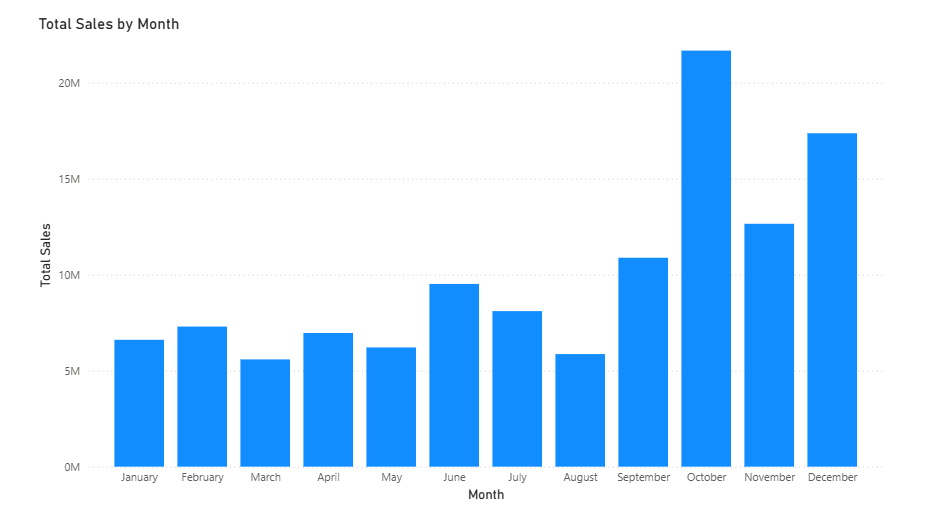
\includegraphics[width=\textwidth, keepaspectratio]{images/sample_sales_by_month.png}
        \caption{Biểu đồ cột (Doanh thu theo Tháng)}
    \end{subfigure}
    \hfill
    \begin{subfigure}{0.48\textwidth}
        \centering
        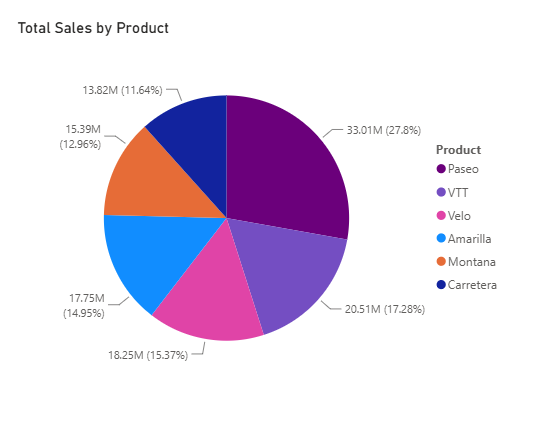
\includegraphics[width=\textwidth, keepaspectratio]{images/sample_sales_by_product.png}
        \caption{Biểu đồ tròn (Cơ cấu theo Sản phẩm)}
    \end{subfigure}
    \caption{Minh họa các biểu đồ cơ bản trên dữ liệu mẫu Financials}
    \label{fig:sample_viz}
\end{figure}

Kết quả thử nghiệm cho thấy Power BI có tốc độ xử lý nhanh, khả năng kéo thả trực quan và đồng bộ hóa bộ lọc tốt giữa các biểu đồ. Đây là tiền đề để nhóm áp dụng vào bộ dữ liệu chính của đồ án.

\newpage

\section{Lựa chọn Dataset và Xây dựng Mô hình Dữ liệu}
\label{sec:data_model}

Chương này dùng để mô tả chi tiết về nguồn gốc bộ dữ liệu, cấu trúc các bảng dữ liệu quan hệ, quy trình tiền xử lý dữ liệu và cách thiết lập mô hình dữ liệu trong Power BI của nhóm.

\subsection{Giới thiệu nguồn dữ liệu và lý do lựa chọn}
\textit{[Hướng dẫn điền: Nhóm tự điền thông tin giới thiệu nguồn dữ liệu mà nhóm đã thống nhất lựa chọn (ví dụ: Kaggle, World Bank, Data.gov...). Nêu rõ lý do lựa chọn bộ dữ liệu này (kích thước dữ liệu, tính thực tiễn, mức độ phong phú của các mối quan hệ giữa các bảng) và cung cấp đường dẫn/liên kết tải dữ liệu công khai].}

\subsection{Mô tả các bảng dữ liệu và trường thông tin quan trọng}
Bộ dữ liệu sử dụng trong đồ án là cơ sở dữ liệu quan hệ (relational dataset) gồm ít nhất 2-3 bảng dữ liệu có liên kết với nhau. Dưới đây là mô tả chi tiết cấu trúc các bảng dữ liệu của nhóm:

\begin{enumerate}
    \item \textbf{Bảng dữ liệu chính (Fact Table - Ví dụ: Bảng giao dịch, bảng sự kiện...)}:
    \begin{itemize}
        \item \texttt{[Tên trường khóa chính]} (Khóa chính): Mã định danh duy nhất của mỗi dòng giao dịch.
        \item \texttt{[Tên trường khóa ngoại]} (Khóa ngoại): Liên kết đến các bảng chiều (Dimension tables).
        \item \texttt{[Tên trường số đo lường]} (Ví dụ: Doanh số, số lượng, điểm số, thời gian...): Các biến định lượng dùng để tính toán chỉ số.
        \item \texttt{[Mô tả các trường thông tin khác...]}
    \end{itemize}
    
    \item \textbf{Bảng dữ liệu chiều thứ nhất (Dimension Table 1 - Ví dụ: Khách hàng, sản phẩm, địa điểm...)}:
    \begin{itemize}
        \item \texttt{[Tên trường khóa chính]} (Khóa chính): Mã định danh duy nhất của thực thể.
        \item \texttt{[Các trường thuộc tính]} (Ví dụ: Tên, phân loại, trạng thái...): Dùng để lọc và phân nhóm dữ liệu.
    \end{itemize}

    \item \textbf{Bảng dữ liệu chiều thứ hai (Dimension Table 2 - Ví dụ: Thời gian, chi nhánh, loại hình...)}:
    \begin{itemize}
        \item \texttt{[Tên trường khóa chính]} (Khóa chính): Mã định danh duy nhất của thực thể.
        \item \texttt{[Các trường thuộc tính]} (Ví dụ: Địa chỉ, vùng miền, danh mục con...): Dùng để lọc và phân nhóm dữ liệu.
    \end{itemize}
    
    \item \textit{[Thêm các bảng khác nếu có...]}
\end{enumerate}

\subsection{Mô hình dữ liệu quan hệ (Data Model) trong Power BI}
Sau khi nạp các bảng dữ liệu vào Power BI Desktop, nhóm tiến hành thiết lập mối quan hệ giữa các bảng (quan hệ một - nhiều $1:\infty$ hoặc một - một $1:1$ thông qua các trường khóa ngoại) để tạo thành mô hình hình sao (Star Schema) hoặc mô hình bông tuyết (Snowflake Schema):

\begin{figure}[H]
    \centering
    % Nhóm sẽ chụp ảnh màn hình Model View thực tế trong Power BI của mình và lưu đè lên file này
    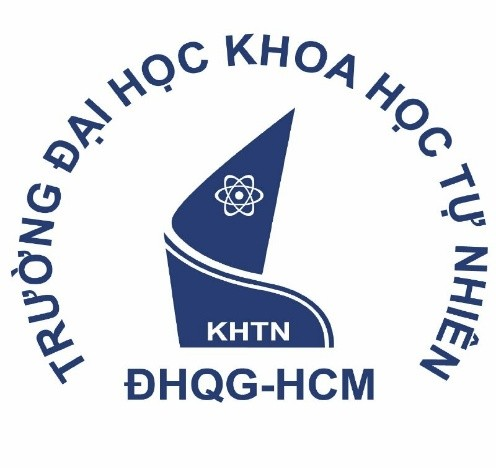
\includegraphics[width=0.85\textwidth, keepaspectratio]{images/data_model_diagram.png}
    \caption{Sơ đồ mối quan hệ (Data Model) thực tế trong Power BI của nhóm}
    \label{fig:data_model}
\end{figure}

\textit{[Nhóm tự điền: Mô tả chi tiết mối quan hệ giữa các bảng đã liên kết. Ví dụ: Bảng A liên kết với bảng B qua trường khóa X với kiểu liên kết một-nhiều và chiều lọc hướng từ A sang B].}

\subsection{Quy trình tiền xử lý dữ liệu (Power Query)}
Dữ liệu thô khi tải về thường chưa sẵn sàng để phân tích ngay, nhóm đã thực hiện quy trình làm sạch và tiền xử lý dữ liệu qua các bước sau trên Power Query Editor:
\begin{enumerate}
    \item \textbf{Xử lý giá trị trống hoặc lỗi (Null/Missing/Error Values)}: \textit{[Mô tả cách xử lý của nhóm, ví dụ: xóa dòng lỗi, điền giá trị trung vị hoặc giá trị mặc định cho ô trống...]}.
    \item \textbf{Chuẩn hóa kiểu dữ liệu (Data Type Correction)}: \textit{[Mô tả cách chuẩn hóa định dạng số, ngày tháng, văn bản để tránh lỗi tính toán và lỗi phân tích địa lý...]}.
    \item \textbf{Biến đổi và trích xuất đặc trưng (Feature Engineering)}: \textit{[Mô tả việc tách/gộp cột, tạo cột mới từ cột cũ, tạo bảng Calendar (bảng Date) bằng DAX hoặc Power Query để hỗ trợ phân tích thời gian...]}.
    \item \textbf{Nối hoặc Gộp các bảng (Append/Merge Queries - Nếu có)}: \textit{[Mô tả cách gộp các file lẻ thành bảng lớn nếu có...]}.
\end{enumerate}
Quá trình tiền xử lý này đảm bảo dữ liệu luôn nhất quán, chính xác, giúp tối ưu hóa hiệu năng tính toán các measure DAX trong Power BI.

\newpage

\section{Xác định Mục tiêu Phân tích}
\label{sec:analysis_goals}

Để báo cáo không bị dàn trải, nhóm giới hạn phạm vi phân tích vào các vụ va chạm giao thông đường bộ tại Great Britain trong giai đoạn \textbf{2020--2024}. Trọng tâm của dashboard là nhận diện các yếu tố thường đi kèm với mức độ nghiêm trọng của tai nạn, thay vì cố gắng phân tích toàn bộ mọi trường dữ liệu trong bộ STATS19.

\subsection{Bài toán phân tích chung của nhóm}

\textbf{Bài toán chung}: Trong giai đoạn 2020--2024, tai nạn giao thông đường bộ tại Great Britain thay đổi như thế nào theo thời gian, điều kiện xảy ra tai nạn, loại phương tiện và đặc điểm người thương vong?

Dashboard của nhóm cần trả lời ngắn gọn ba câu hỏi chính:

\begin{itemize}
    \item Số vụ va chạm và số người thương vong biến động ra sao theo thời gian?
    \item Những điều kiện đường sá, thời tiết, ánh sáng hoặc tốc độ nào thường đi kèm với tai nạn nghiêm trọng?
    \item Nhóm phương tiện và nhóm người tham gia giao thông nào có rủi ro thương vong cao hơn?
\end{itemize}

\subsection{Mục tiêu phân tích cụ thể của từng thành viên}

Mỗi thành viên phụ trách một góc nhìn nhỏ, có thể trình bày bằng một cụm biểu đồ ngắn trong báo cáo và một phần trên dashboard tổng hợp.

\begin{enumerate}
    \item \textbf{Lê Lâm Trí Đức -- Tổng quan và xu hướng thời gian}
    
    Phân tích số vụ va chạm, số phương tiện liên quan và số người thương vong theo năm, tháng, ngày trong tuần và giờ trong ngày. Mục tiêu là xác định giai đoạn hoặc khung thời gian có số vụ tai nạn cao bất thường.

    \item \textbf{Hoàng Quốc Việt -- Điều kiện đường sá và môi trường}
    
    So sánh số vụ tai nạn và mức độ nghiêm trọng theo loại đường, giới hạn tốc độ, điều kiện ánh sáng, thời tiết và mặt đường. Mục tiêu là nhận diện những bối cảnh môi trường có tỷ lệ tai nạn nghiêm trọng cao.

    \item \textbf{Nguyễn Lê Thế Vinh -- Phương tiện và người lái}
    
    Phân tích tai nạn theo loại phương tiện, độ tuổi người lái, giới tính người lái và thao tác di chuyển của phương tiện. Mục tiêu là xác định nhóm phương tiện hoặc nhóm người lái xuất hiện nhiều trong các vụ tai nạn nghiêm trọng.

    \item \textbf{Phạm Quang Vinh -- Người thương vong và nhóm rủi ro}
    
    Phân tích mức độ thương vong theo nhóm tuổi, giới tính, vai trò tham gia giao thông và loại đối tượng thương vong. Mục tiêu là chỉ ra nhóm người tham gia giao thông cần được chú ý hơn trong các khuyến nghị an toàn.
\end{enumerate}

Với cách chia này, các mục tiêu đủ nhỏ để triển khai trong phạm vi báo cáo thực hành, đồng thời vẫn liên kết trực tiếp với bài toán chung về mức độ nghiêm trọng và rủi ro tai nạn giao thông.

\newpage

\section{Phân tích Dữ liệu và Trực quan hóa}
\label{sec:visualization}

Chương này trình bày chi tiết các biểu đồ phân tích và diễn giải kết quả cho bốn mục tiêu đã xác định ở Chương~\ref{sec:analysis_goals}. Các biểu đồ được thiết kế trực quan bằng Vega-Lite/Deneb kết hợp với các bộ lọc tương tác để làm nổi bật những phát hiện quan trọng nhất.

\subsection{Tổng quan và xu hướng thời gian}

\textbf{Mục tiêu}: Phân tích sự biến động của tổng số vụ va chạm trong giai đoạn 2020--2024, đồng thời xác định các khung thời gian có tần suất tai nạn cao bất thường.

\textbf{Biểu đồ thực tế}:
\begin{itemize}
    \item Biểu đồ cột xếp chồng (Stacked Bar Chart): Thể hiện tổng số vụ va chạm theo từng năm, phân loại theo khu vực Thành thị/Nông thôn.
    \item Biểu đồ bản đồ nhiệt (Heatmap Matrix): Thể hiện mật độ số vụ va chạm theo từng thứ trong tuần và khung giờ trong ngày (00:00 -- 23:00).
    \item Biểu đồ cột (Bar Chart): Thể hiện biến động tổng số vụ va chạm theo từng tháng trong năm.
    \item Biểu đồ đường (Line Chart): Thể hiện xu hướng tai nạn phân theo mức độ nghiêm trọng (Tử vong, Nghiêm trọng, Nhẹ) qua các năm 2020--2024.
\end{itemize}

\textbf{Nhận xét rút ra từ dữ liệu}:
\begin{itemize}
    \item \textbf{Xu hướng theo năm và khu vực}: Tổng số vụ va chạm tăng mạnh từ 2020 và đạt đỉnh vào 2022, sau đó có dấu hiệu giảm nhẹ về năm 2024. Đáng chú ý, các vụ tai nạn diễn ra ở khu vực Thành thị (màu xanh sáng) luôn chiếm tỷ trọng lớn hơn hẳn so với khu vực Nông thôn.
    \item \textbf{Mật độ va chạm theo Thứ và Giờ}: Tai nạn tập trung dày đặc vào các ngày làm việc trong tuần (Thứ 2 đến Thứ 6). Đỉnh điểm rủi ro rơi vào khung giờ tan tầm buổi chiều từ 15h00 đến 18h00 (đậm nhất ở dải 16h00 -- 17h00), tương đồng với thời gian lưu lượng giao thông đông đúc. Vào cuối tuần, mật độ tai nạn giảm đi rõ rệt.
    \item \textbf{Biến động theo tháng}: Tần suất va chạm có dấu hiệu tăng cao hơn vào những tháng cuối năm (từ Tháng 9 đến Tháng 11). Tháng 10 thường là tháng ghi nhận số lượng tai nạn cao nhất, có thể liên quan đến điều kiện thời tiết bắt đầu chuyển mùa.
    \item \textbf{Mức độ nghiêm trọng khá ổn định}: Mặc dù tổng số vụ va chạm biến động qua các năm, tỷ trọng các vụ ở mức độ Nhẹ vẫn chiếm áp đảo tuyệt đối. Đường xu hướng của các vụ án Tử vong (màu đỏ) và Nghiêm trọng (màu vàng) duy trì khá phẳng và ổn định, cho thấy mức độ thảm khốc không tăng đột biến so với mức tăng của tổng số vụ tai nạn chung.
\end{itemize}

\begin{figure}[H]
    \centering
    \begin{subfigure}{0.48\textwidth}
        \centering
        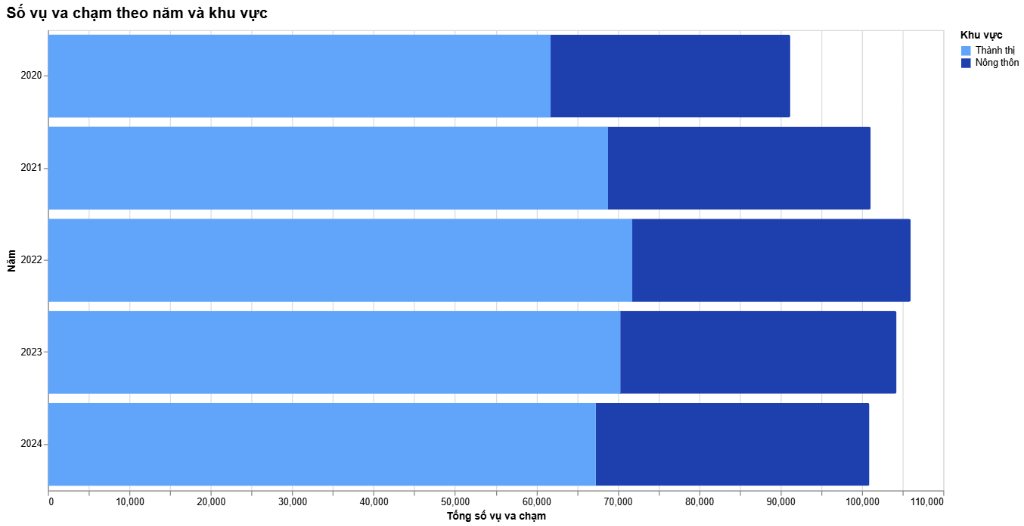
\includegraphics[width=\textwidth, keepaspectratio]{images/memberA_year_area.png}
        \caption{Số vụ theo năm và khu vực}
    \end{subfigure}
    \hfill
    \begin{subfigure}{0.48\textwidth}
        \centering
        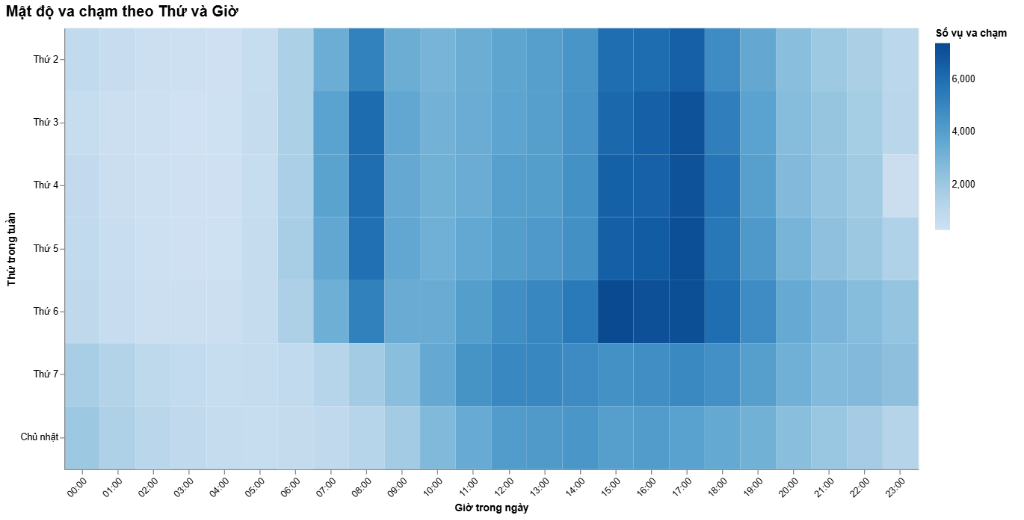
\includegraphics[width=\textwidth, keepaspectratio]{images/memberA_heatmap.png}
        \caption{Mật độ va chạm theo Thứ và Giờ}
    \end{subfigure}

    \vspace{0.3cm}

    \begin{subfigure}{0.48\textwidth}
        \centering
        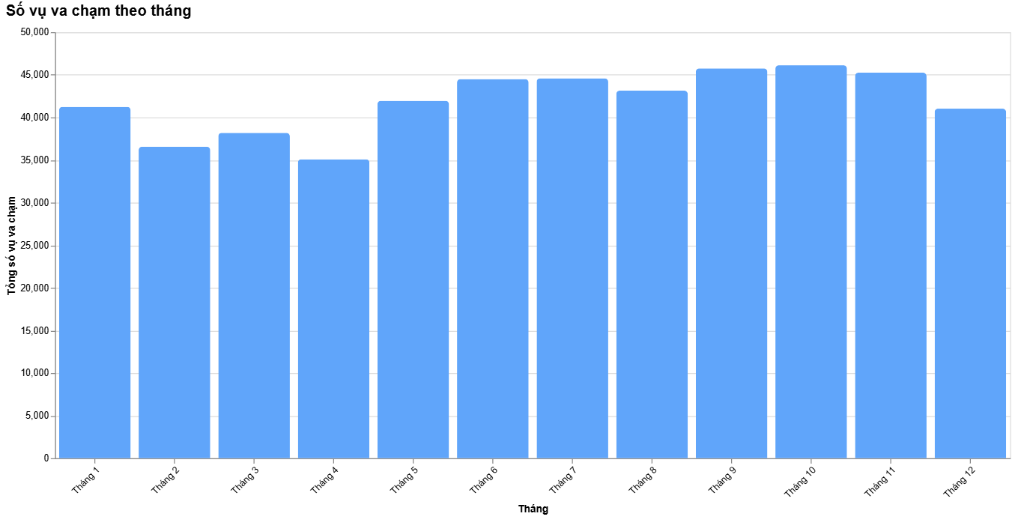
\includegraphics[width=\textwidth, keepaspectratio]{images/memberA_month.png}
        \caption{Số vụ va chạm theo tháng}
    \end{subfigure}
    \hfill
    \begin{subfigure}{0.48\textwidth}
        \centering
        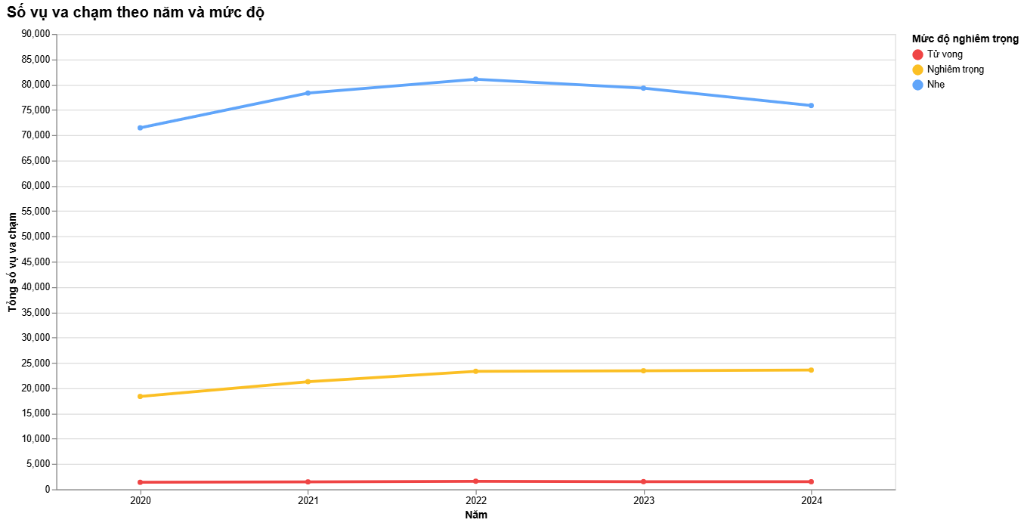
\includegraphics[width=\textwidth, keepaspectratio]{images/memberA_year_severity.png}
        \caption{Số vụ theo năm và mức độ}
    \end{subfigure}
    \caption{Các biểu đồ phân tích Tổng quan và xu hướng thời gian}
    \label{fig:memberA_charts}
\end{figure}

\subsection{Điều kiện đường sá và môi trường}


\textbf{Mục tiêu}: Phân tích sự ảnh hưởng của các điều kiện môi trường (thời tiết, ánh sáng) và đặc điểm hạ tầng (tình trạng mặt đường, loại đường, giới hạn tốc độ) đối với số lượng và mức độ nghiêm trọng của các vụ va chạm.

\textbf{Biểu đồ thực tế}:
\begin{itemize}
    \item Biểu đồ cột nhóm (Grouped Bar Chart): Thể hiện tổng số vụ va chạm theo tình trạng mặt đường, phân tách theo khu vực (Thành thị/Nông thôn).
    \item Biểu đồ bản đồ nhiệt (Heatmap Matrix): Thể hiện số vụ va chạm theo sự kết hợp giữa các điều kiện thời tiết và ánh sáng.
    \item Biểu đồ cột (Bar Chart): So sánh số lượng các vụ tai nạn diễn ra trên các tuyến đường có mức giới hạn tốc độ khác nhau.
    \item Biểu đồ cột xếp chồng (Stacked Bar Chart): Thể hiện số vụ va chạm phân bổ theo loại đường, phân lớp theo mức độ nghiêm trọng.
\end{itemize}

\textbf{Nhận xét rút ra từ dữ liệu}:
\begin{itemize}
    \item \textbf{Tình trạng mặt đường và Khu vực}: Hầu hết các vụ va chạm xảy ra trong điều kiện mặt đường "Khô ráo" ở khu vực "Thành thị" (khoảng 250 nghìn vụ). Mặc dù vậy, nhóm điều kiện "Ẩm ướt" vẫn ghi nhận một số lượng đáng kể tai nạn, cho thấy mặt đường trơn trượt vẫn là một rủi ro lớn. Ở hầu hết các tình trạng mặt đường, tai nạn tại khu vực Thành thị luôn chiếm ưu thế so với Nông thôn.
    \item \textbf{Thời tiết và Ánh sáng}: Tổ hợp có số vụ tai nạn cao nhất (thể hiện bằng ô màu xanh đậm nhất) là "Nắng (không gió)" kết hợp với "Ban ngày" với gần 300 nghìn vụ. Điều này hợp lý bởi đây là thời điểm lưu lượng xe cộ lưu thông đông nhất. Tổ hợp rủi ro lớn thứ hai là "Nắng (không gió)" đi kèm với "Tối (có đèn)". Các điều kiện thời tiết khắc nghiệt (Mưa, Tuyết, Sương mù) có số vụ va chạm tuyệt đối thấp hơn do người dân hạn chế ra đường.
    \item \textbf{Giới hạn tốc độ}: Đường có giới hạn tốc độ 30 mph (đặc trưng cho đường nội đô) ghi nhận số lượng tai nạn kỷ lục, vượt mốc 260 nghìn vụ. Đứng thứ hai là các cung đường giới hạn 20 mph (khoảng 80 nghìn vụ), và thứ ba là đường quốc lộ/ngoại ô giới hạn 60 mph. Điều này phản ánh thực tế rằng tai nạn dễ xảy ra hơn trong môi trường giao thông chằng chịt ở nội thành, dù tốc độ di chuyển không quá lớn.
    \item \textbf{Loại đường và mức độ nghiêm trọng}: Đường đơn (Single carriageway) chứng kiến số lượng tai nạn áp đảo hoàn toàn so với các loại hình khác như Đường đôi hay Vòng xuyến. Không những thế, tỷ lệ các vụ tai nạn dẫn đến chấn thương Nghiêm trọng (Serious - màu vàng) và Tử vong (Fatal - màu đỏ) trên đường đơn cũng chiếm một diện tích lớn trên thân cột, báo động về mức độ nguy hiểm của loại hạ tầng thiếu dải phân cách này.
\end{itemize}

\begin{figure}[H]
    \centering
    \begin{subfigure}{0.48\textwidth}
        \centering
        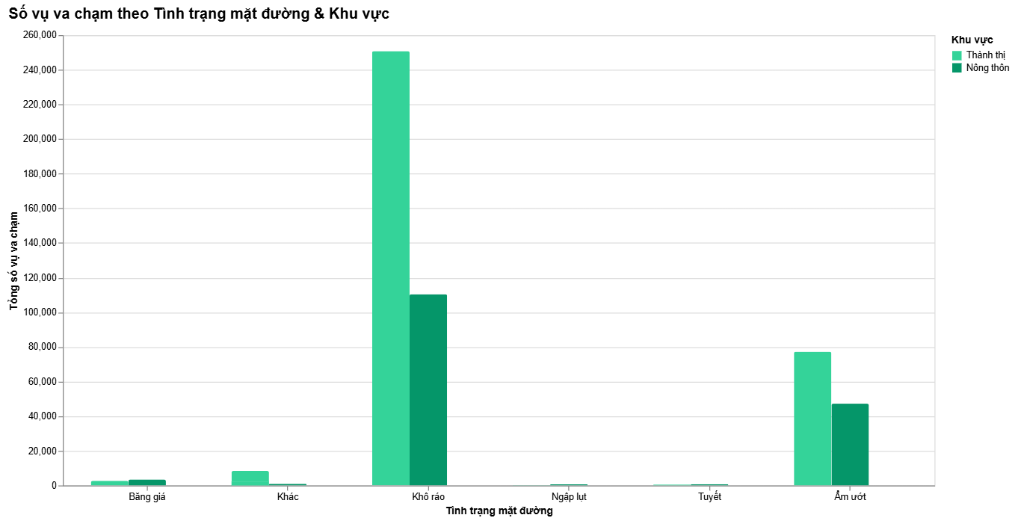
\includegraphics[width=\textwidth, keepaspectratio]{images/memberB_surface_area.png}
        \caption{Mặt đường và Khu vực}
    \end{subfigure}
    \hfill
    \begin{subfigure}{0.48\textwidth}
        \centering
        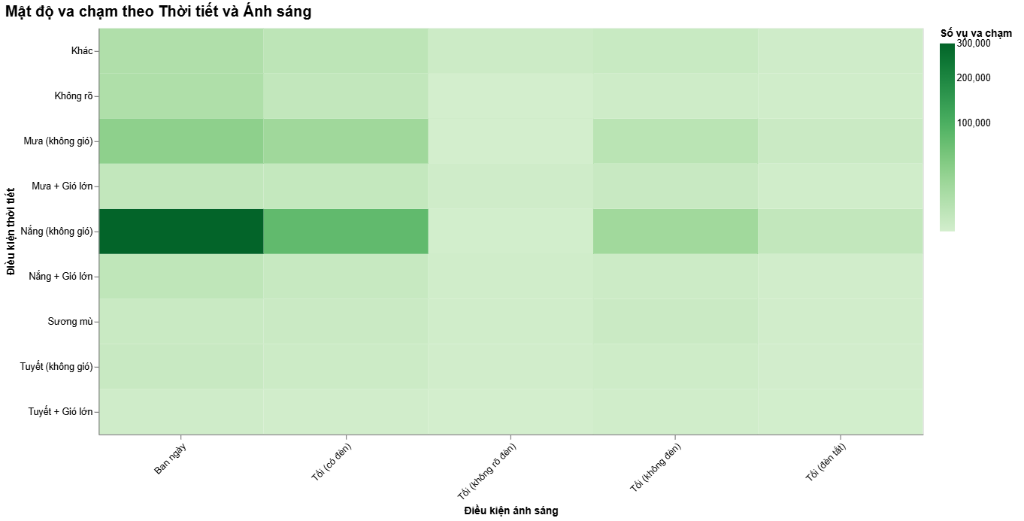
\includegraphics[width=\textwidth, keepaspectratio]{images/memberB_weather_light.png}
        \caption{Thời tiết và Ánh sáng}
    \end{subfigure}

    \vspace{0.3cm}

    \begin{subfigure}{0.48\textwidth}
        \centering
        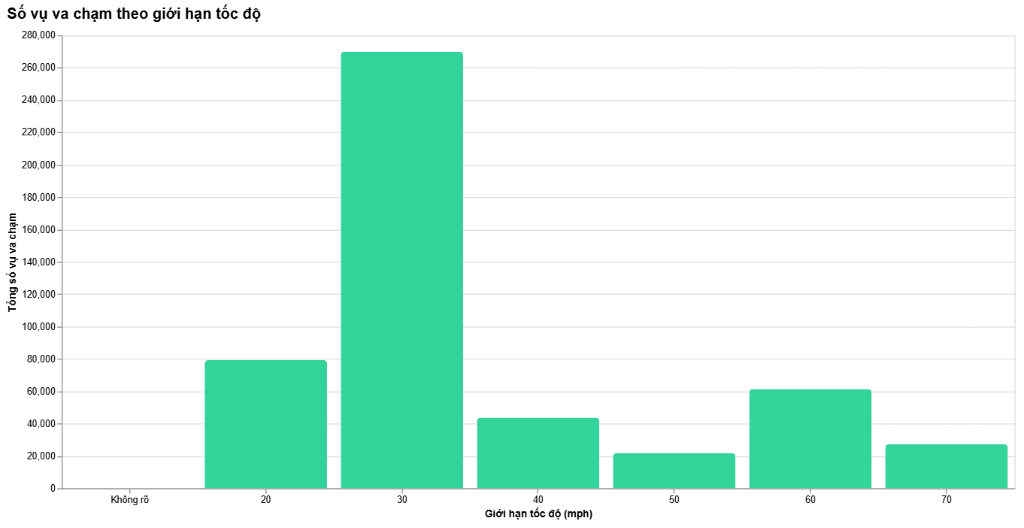
\includegraphics[width=\textwidth, keepaspectratio]{images/memberB_speed_limit.png}
        \caption{Va chạm theo giới hạn tốc độ}
    \end{subfigure}
    \hfill
    \begin{subfigure}{0.48\textwidth}
        \centering
        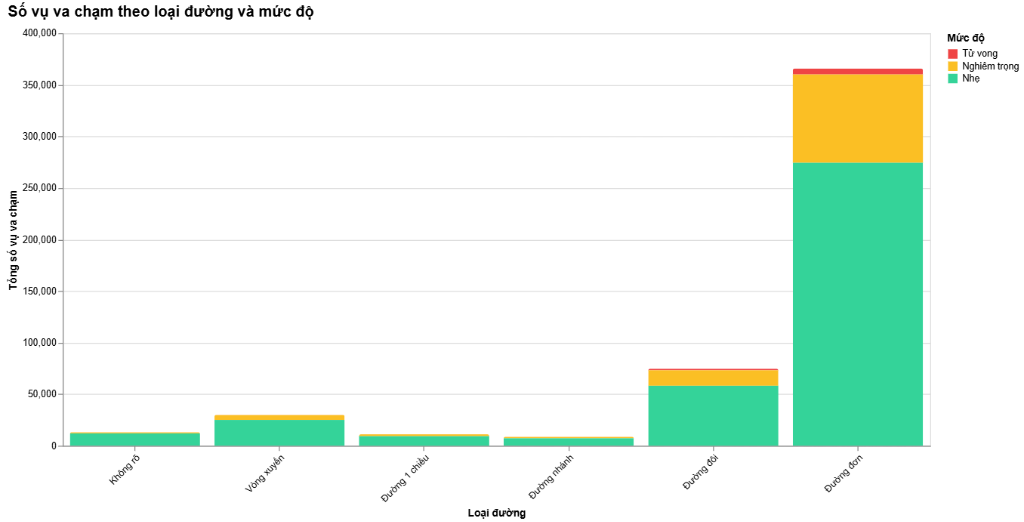
\includegraphics[width=\textwidth, keepaspectratio]{images/memberB_road_type.png}
        \caption{Loại đường và mức độ}
    \end{subfigure}
    \caption{Các biểu đồ phân tích Điều kiện đường sá và môi trường}
    \label{fig:memberB_charts}
\end{figure}

\subsection{Phương tiện và người lái}

\textbf{Mục tiêu}: Phân tích đặc điểm phương tiện và người lái trong các vụ va chạm, từ đó nhận diện nhóm phương tiện hoặc nhóm người lái xuất hiện nhiều trong các vụ tai nạn nghiêm trọng.

\textbf{Biểu đồ thực tế}:
\begin{itemize}
    \item Biểu đồ cột ngang (Bar chart): Thể hiện Top 10 loại phương tiện xuất hiện nhiều nhất trong các vụ va chạm.
    \item Biểu đồ vòng (Donut chart): Thể hiện tỷ lệ phương tiện tham gia va chạm theo khu vực Thành thị/Nông thôn.
    \item Biểu đồ cột xếp chồng (Stacked Column Chart): So sánh số phương tiện theo nhóm tuổi và giới tính người lái.
    \item Biểu đồ kết hợp cột và đường (Combo Chart): Đối chiếu số lượng phương tiện với số ca thương vong nặng theo nhóm tuổi.
\end{itemize}

\textbf{Nhận xét rút ra từ dữ liệu}:
\begin{itemize}
    \item \textbf{Ô tô chiếm ưu thế rất rõ}: Trong Top 10 loại phương tiện, nhóm Car vượt xa toàn bộ các nhóm còn lại. Các nhóm đứng sau như xe đạp, xe tải nhẹ và xe máy có số lượng thấp hơn nhiều, vì vậy khi đọc biểu đồ cần xem ô tô như nhóm nền chính của bức tranh va chạm.
    \item \textbf{Va chạm tập trung nhiều hơn ở Thành thị}: Biểu đồ vòng cho thấy khu vực Thành thị chiếm khoảng hai phần ba tổng số phương tiện liên quan đến va chạm, trong khi Nông thôn chiếm khoảng một phần ba. Chênh lệch này khá dễ hiểu nếu nhìn từ mật độ phương tiện và tần suất di chuyển trong khu vực đô thị.
    \item \textbf{Nhóm 26--35 tuổi nổi bật nhất}: Ở biểu đồ tuổi và giới tính, nhóm 26--35 có số phương tiện cao nhất, sau đó giảm dần qua các nhóm 36--45 và 46--55. Đây là nhóm tuổi tham gia giao thông thường xuyên, nên biểu đồ cho thấy họ xuất hiện nhiều trong các vụ va chạm hơn các nhóm quá trẻ hoặc cao tuổi.
    \item \textbf{Nam giới luôn cao hơn nữ giới ở hầu hết nhóm tuổi}: Các cột màu xanh của nam giới cao hơn rõ so với cột màu hồng ở gần như toàn bộ các nhóm tuổi. Đường thương vong nặng trong biểu đồ kết hợp cũng đạt đỉnh ở nhóm 26--35, rồi giảm dần ở các nhóm tuổi lớn hơn, khá tương đồng với xu hướng số phương tiện.
\end{itemize}

\begin{figure}[H]
    \centering
    \begin{subfigure}{0.48\textwidth}
        \centering
        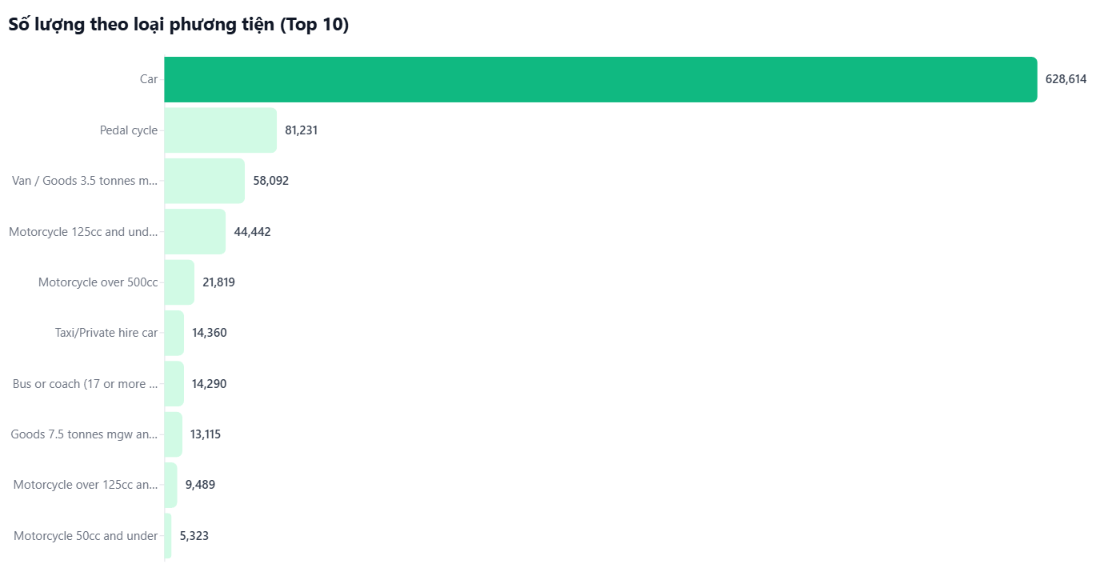
\includegraphics[width=\textwidth, keepaspectratio]{images/memberC_vehicle_type_top10.png}
        \caption{Top 10 loại phương tiện}
    \end{subfigure}
    \hfill
    \begin{subfigure}{0.48\textwidth}
        \centering
        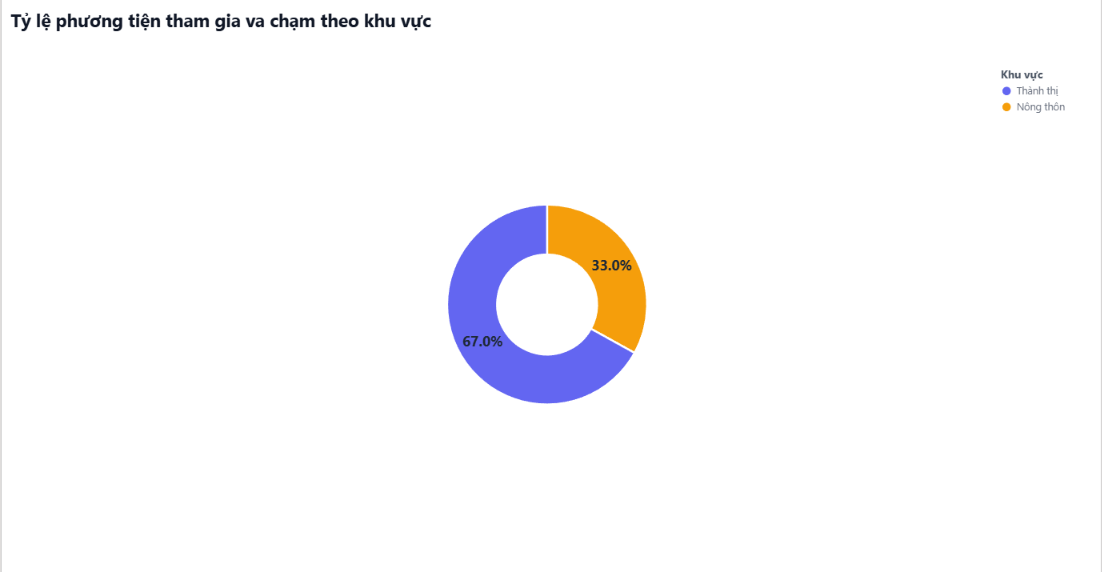
\includegraphics[width=\textwidth, keepaspectratio]{images/memberC_urban_rural_ratio.png}
        \caption{Tỷ lệ phương tiện theo khu vực}
    \end{subfigure}

    \vspace{0.3cm}

    \begin{subfigure}{0.48\textwidth}
        \centering
        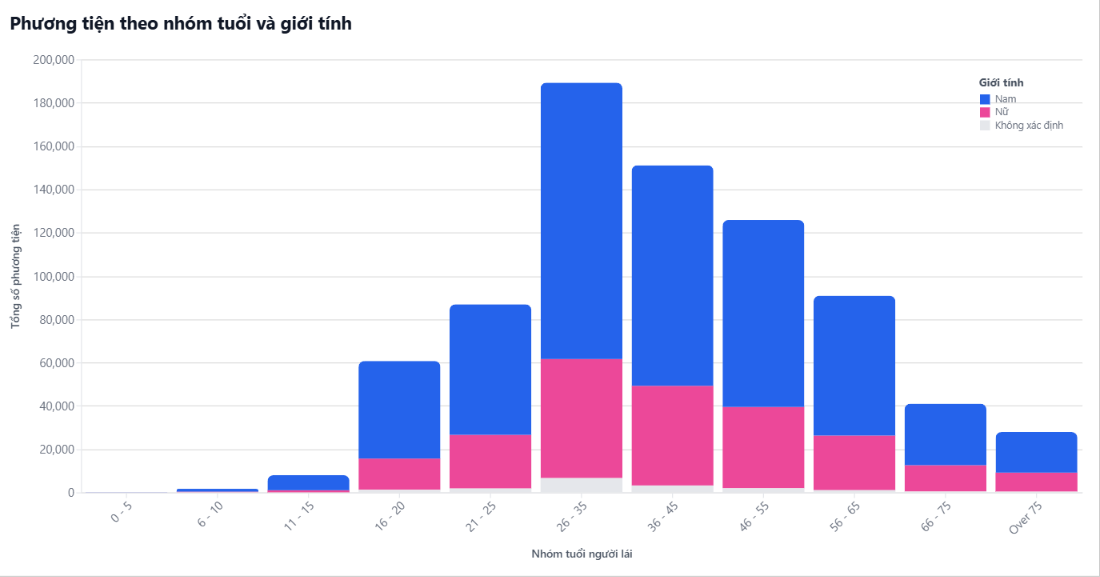
\includegraphics[width=\textwidth, keepaspectratio]{images/memberC_driver_age_gender.png}
        \caption{Nhóm tuổi và giới tính người lái}
    \end{subfigure}
    \hfill
    \begin{subfigure}{0.48\textwidth}
        \centering
        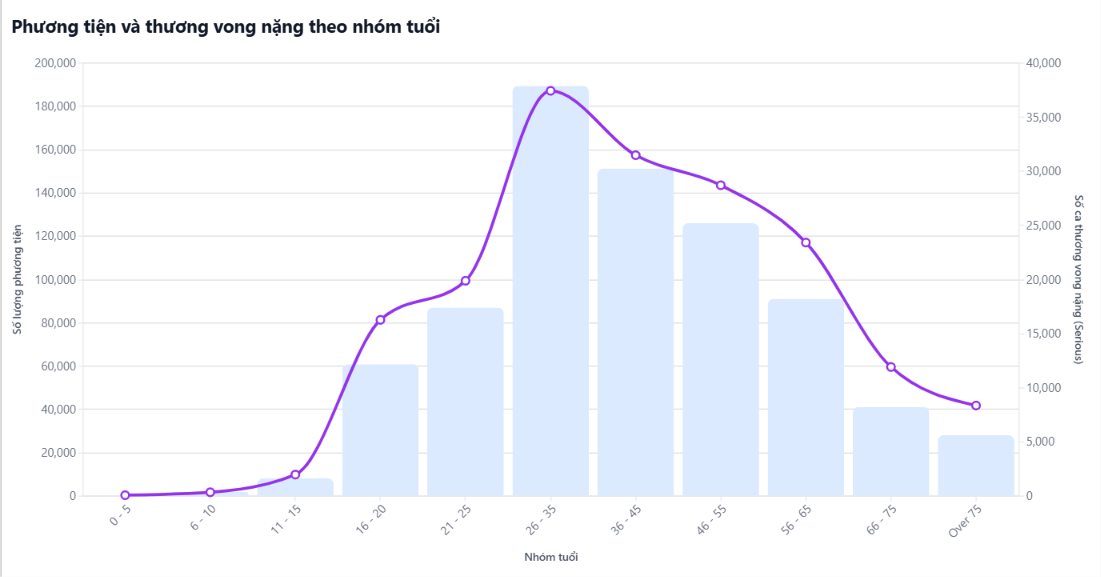
\includegraphics[width=\textwidth, keepaspectratio]{images/memberC_age_severe_casualties.png}
        \caption{Phương tiện và thương vong nặng theo tuổi}
    \end{subfigure}
    \caption{Các biểu đồ phân tích Phương tiện và người lái}
    \label{fig:memberC_charts}
\end{figure}

\subsection{Người thương vong và nhóm rủi ro}

\textbf{Mục tiêu}: Phân tích đặc điểm người thương vong theo độ tuổi, giới tính, vai trò tham gia giao thông và mức độ thương vong để xác định các nhóm rủi ro cao.

\textbf{Biểu đồ thực tế}:
\begin{itemize}
    \item Biểu đồ cột ngang (Bar chart): So sánh số người thương vong theo vai trò tham gia giao thông.
    \item Biểu đồ cột xếp chồng (Stacked Bar Chart): Thể hiện số người thương vong theo nhóm tuổi và mức độ nghiêm trọng.
    \item Biểu đồ cột nhóm (Clustered Column Chart): So sánh số người thương vong theo nhóm tuổi và giới tính.
    \item Biểu đồ cột 100\% xếp chồng (100\% Stacked Column Chart): So sánh tỷ lệ mức độ thương vong theo vai trò tham gia giao thông.
\end{itemize}

\textbf{Nhận xét rút ra từ dữ liệu}:
\begin{itemize}
    \item \textbf{Người điều khiển phương tiện chiếm nhiều nhất về số lượng}: Biểu đồ theo vai trò cho thấy nhóm Người điều khiển có số người thương vong lớn hơn hẳn Hành khách và Người đi bộ. Đây là nhóm trực tiếp tham gia điều khiển phương tiện, nên cũng là nhóm xuất hiện dày nhất trong thống kê thương vong.
    \item \textbf{Nhóm tuổi 26--35 là nhóm nổi bật nhất}: Khi phân theo tuổi và mức độ, nhóm 26--35 có tổng số thương vong cao nhất. Các nhóm 36--45 và 46--55 cũng còn ở mức cao, trong khi trẻ em và nhóm trên 66 tuổi thấp hơn rõ rệt về số lượng tuyệt đối.
    \item \textbf{Thương vong nhẹ vẫn chiếm phần lớn}: Ở hầu hết nhóm tuổi, phần màu xanh của mức độ Nhẹ là phần dài nhất trên thanh. Tuy vậy, phần Nghiêm trọng và Tử vong vẫn xuất hiện đều ở các nhóm tuổi trưởng thành, nên không thể chỉ nhìn tổng số cao mà bỏ qua mức độ hậu quả.
    \item \textbf{Người đi bộ có tỷ lệ hậu quả nặng đáng chú ý}: Nếu xét theo tỷ lệ, Người đi bộ có phần Nghiêm trọng và Tử vong lớn hơn hai nhóm còn lại. Nói cách khác, Người điều khiển là nhóm đông nhất về số lượng thương vong, nhưng Người đi bộ lại là nhóm cần chú ý nhiều hơn khi đánh giá mức độ nghiêm trọng.
    \item \textbf{Nam giới cao hơn nữ giới ở hầu hết nhóm tuổi}: Biểu đồ giới tính cho thấy cột Nam luôn cao hơn cột Nữ, đặc biệt rõ ở các nhóm tuổi 26--35, 36--45 và 46--55. Ở các nhóm tuổi cao hơn, khoảng cách này thu hẹp lại nhưng vẫn giữ cùng chiều hướng.
\end{itemize}

\begin{figure}[H]
    \centering
    \begin{subfigure}{0.48\textwidth}
        \centering
        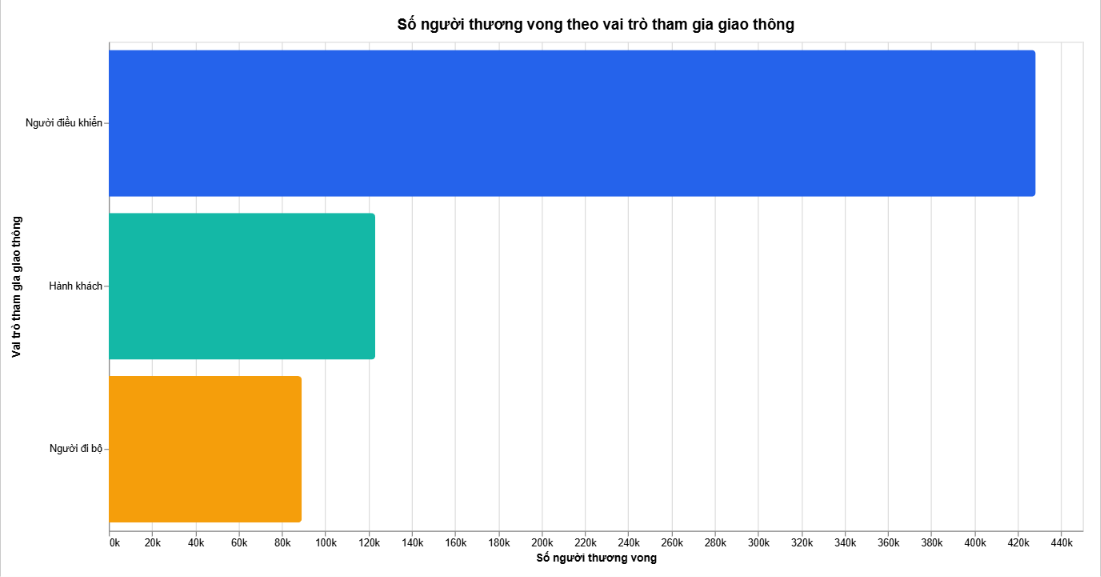
\includegraphics[width=\textwidth, keepaspectratio]{images/memberD_casualties_by_role.png}
        \caption{Thương vong theo vai trò}
    \end{subfigure}
    \hfill
    \begin{subfigure}{0.48\textwidth}
        \centering
        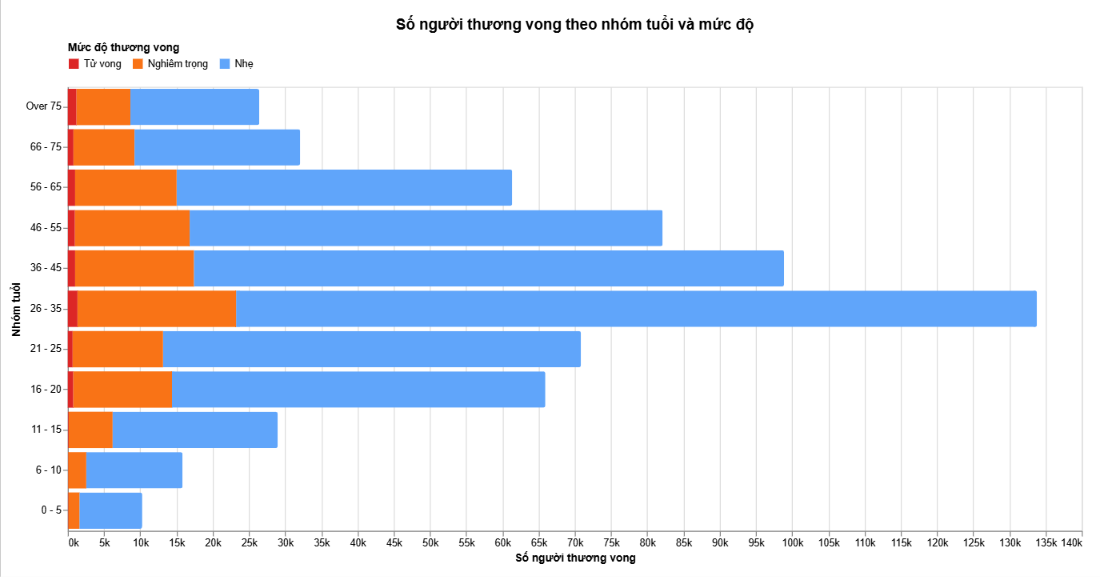
\includegraphics[width=\textwidth, keepaspectratio]{images/memberD_age_severity.png}
        \caption{Nhóm tuổi và mức độ thương vong}
    \end{subfigure}

    \vspace{0.3cm}

    \begin{subfigure}{0.48\textwidth}
        \centering
        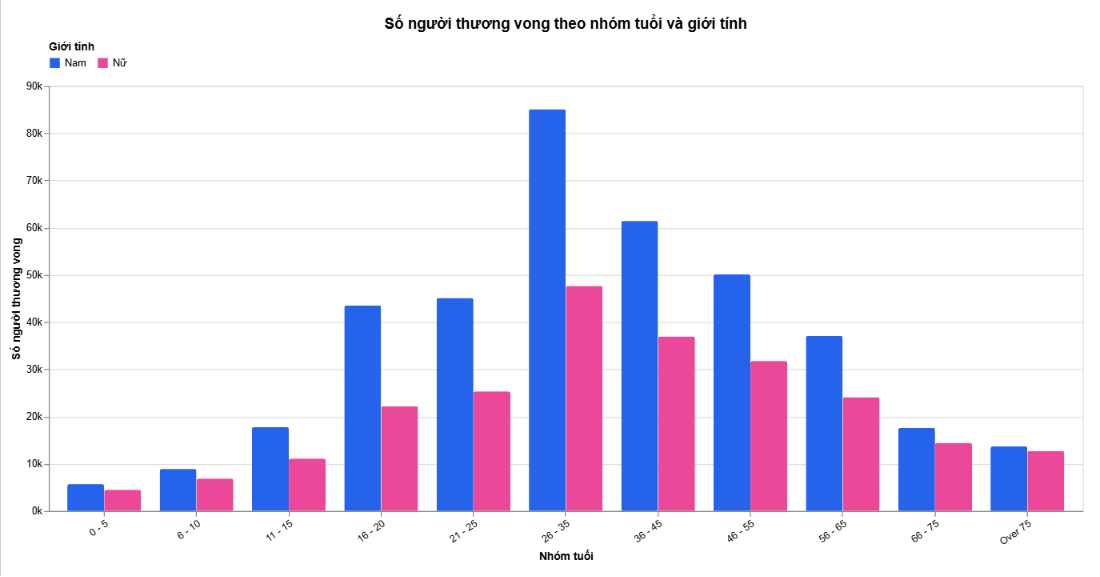
\includegraphics[width=\textwidth, keepaspectratio]{images/memberD_age_gender.png}
        \caption{Nhóm tuổi và giới tính}
    \end{subfigure}
    \hfill
    \begin{subfigure}{0.48\textwidth}
        \centering
        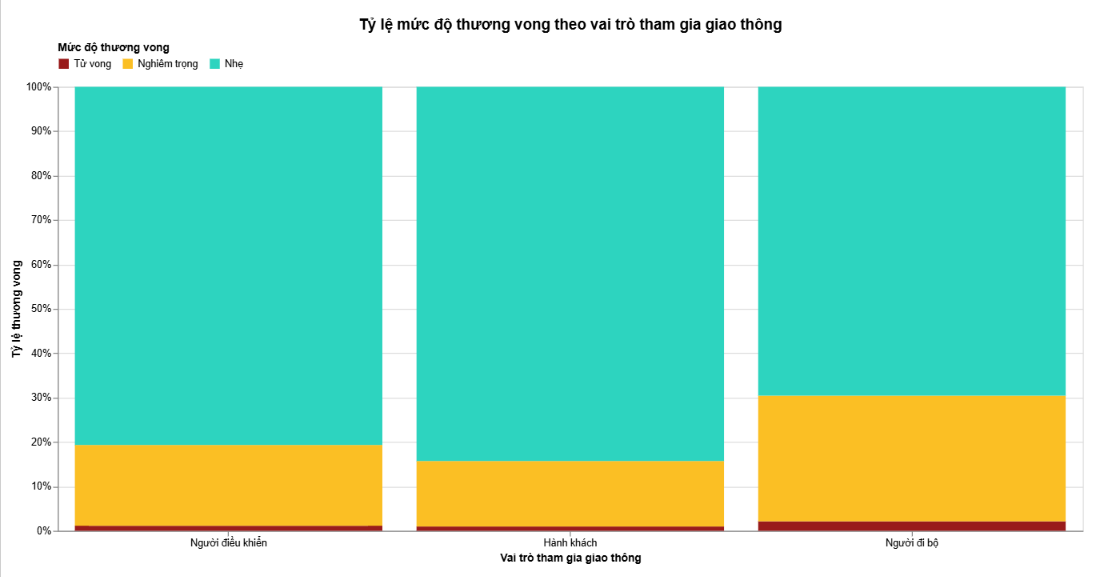
\includegraphics[width=\textwidth, keepaspectratio]{images/memberD_role_severity_ratio.png}
        \caption{Tỷ lệ mức độ theo vai trò}
    \end{subfigure}
    \caption{Các biểu đồ phân tích Người thương vong và nhóm rủi ro}
    \label{fig:memberD_charts}
\end{figure}

\subsection{Giao diện dashboard tổng hợp}

Sau khi hoàn thành các biểu đồ thành phần, nhóm đã tổng hợp và xây dựng một hệ thống dashboard tương tác gồm 5 trang báo cáo chuyên sâu trong Power BI. Hệ thống dashboard được thiết kế nhất quán với thanh điều hướng (navigation bar) ở bên trái, hàng thẻ KPI tổng hợp ở trên cùng, các bộ lọc (slicers) Dropdown ở góc trên bên phải và lưới biểu đồ chi tiết ở trung tâm.

Dưới đây là chi tiết giao diện thực tế của 5 trang báo cáo đã được hoàn thiện:

\begin{figure}[H]
    \centering
    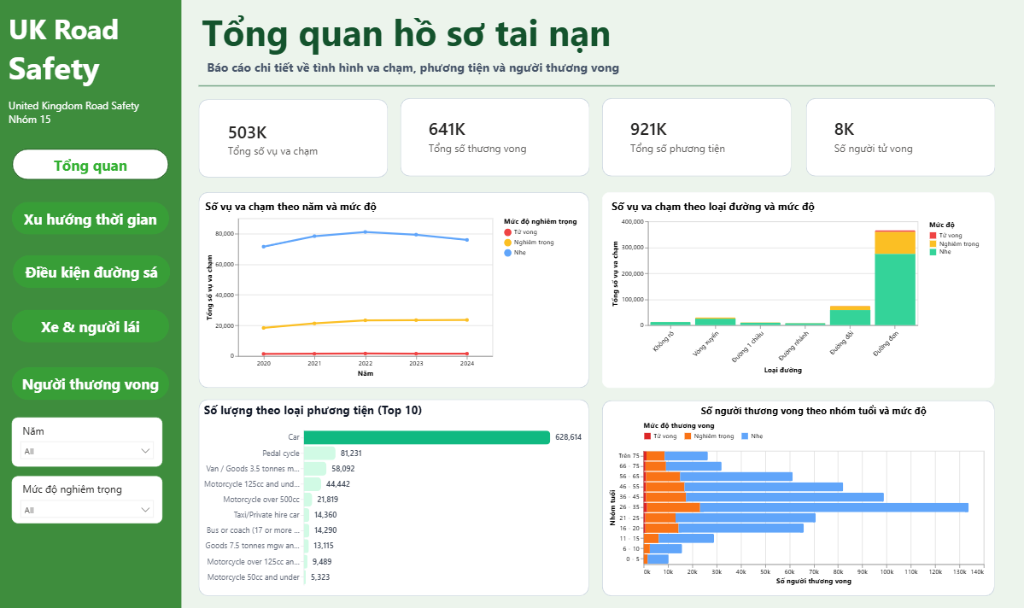
\includegraphics[width=0.75\textwidth, keepaspectratio]{images/dashboard_page1.png}
    \caption{Tổng quan hồ sơ tai nạn}
    \label{fig:dashboard_page1}
\end{figure}

\textbf{Tổng quan hồ sơ tai nạn} (Hình~\ref{fig:dashboard_page1}) cung cấp cái nhìn toàn cảnh về quy mô dữ liệu với 4 thẻ KPI chính: tổng số vụ va chạm (503K), tổng số thương vong (641K), tổng số phương tiện liên quan (921K) và số người tử vong (8K). Đồng thời tích hợp các biểu đồ quan trọng nhất từ các mục tiêu để người quản trị có góc nhìn bao quát tức thì.

\begin{figure}[H]
    \centering
    \begin{subfigure}[t]{0.48\textwidth}
        \centering
        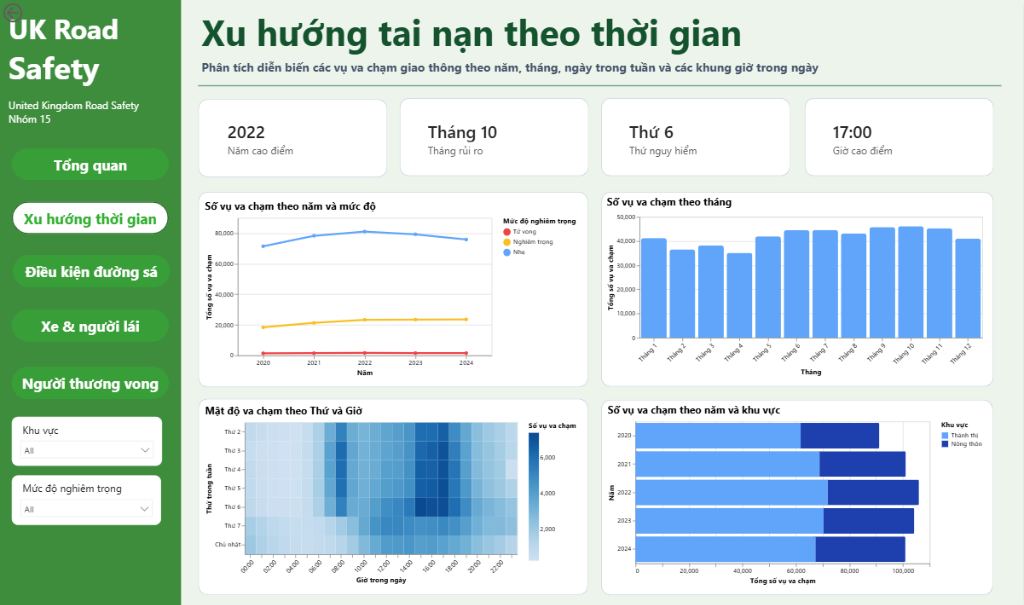
\includegraphics[width=\textwidth, keepaspectratio]{images/dashboard_page2.png}
        \caption{Xu hướng thời gian}
        \label{fig:dashboard_page2}
    \end{subfigure}
    \hfill
    \begin{subfigure}[t]{0.48\textwidth}
        \centering
        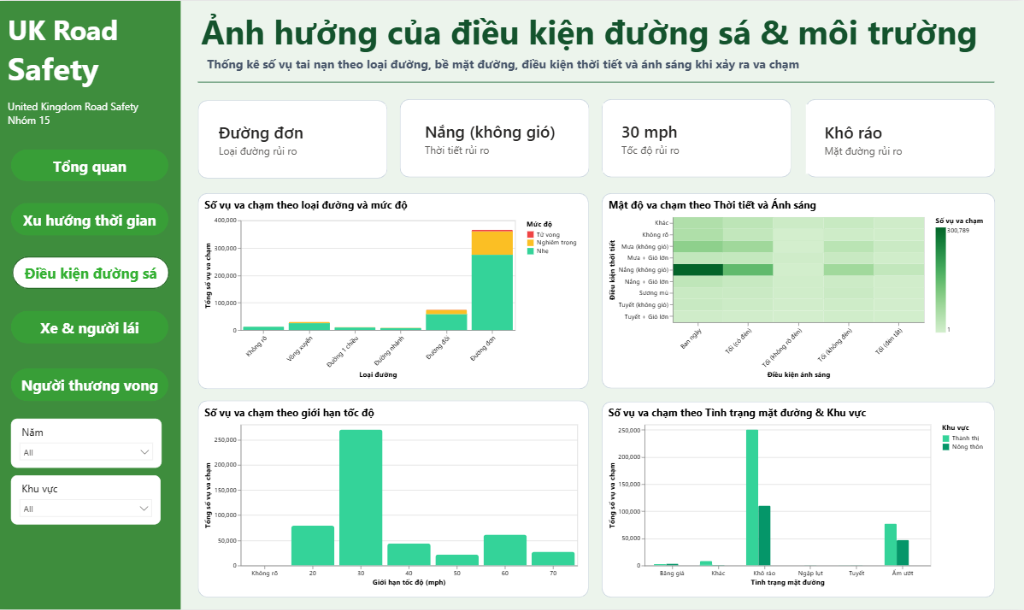
\includegraphics[width=\textwidth, keepaspectratio]{images/dashboard_page3.png}
        \caption{Điều kiện đường sá và môi trường}
        \label{fig:dashboard_page3}
    \end{subfigure}
    \caption{Giao diện trang Xu hướng thời gian và Điều kiện đường sá}
    \label{fig:dashboard_group1}
\end{figure}

\textbf{Phân tích xu hướng tai nạn theo thời gian} (Hình~\ref{fig:dashboard_page2}) tập trung vào làm rõ các mốc thời gian xảy ra tai nạn. Các thẻ KPI làm nổi bật các đỉnh điểm rủi ro: năm cao điểm (2022), tháng rủi ro (tháng 10), ngày nguy hiểm nhất trong tuần (thứ 6) và giờ cao điểm va chạm (17:00).

\textbf{Ảnh hưởng của điều kiện đường sá và môi trường} (Hình~\ref{fig:dashboard_page3}) phân tích các yếu tố hạ tầng và ngoại cảnh. Thẻ KPI thể hiện các điều kiện ghi nhận số tai nạn lớn nhất: loại đường đơn rủi ro nhất (Single carriageway), thời tiết nắng ấm (Fine no high winds), giới hạn tốc độ nội đô (30 mph) và tình trạng mặt đường khô ráo (Dry).

\begin{figure}[H]
    \centering
    \begin{subfigure}[t]{0.48\textwidth}
        \centering
        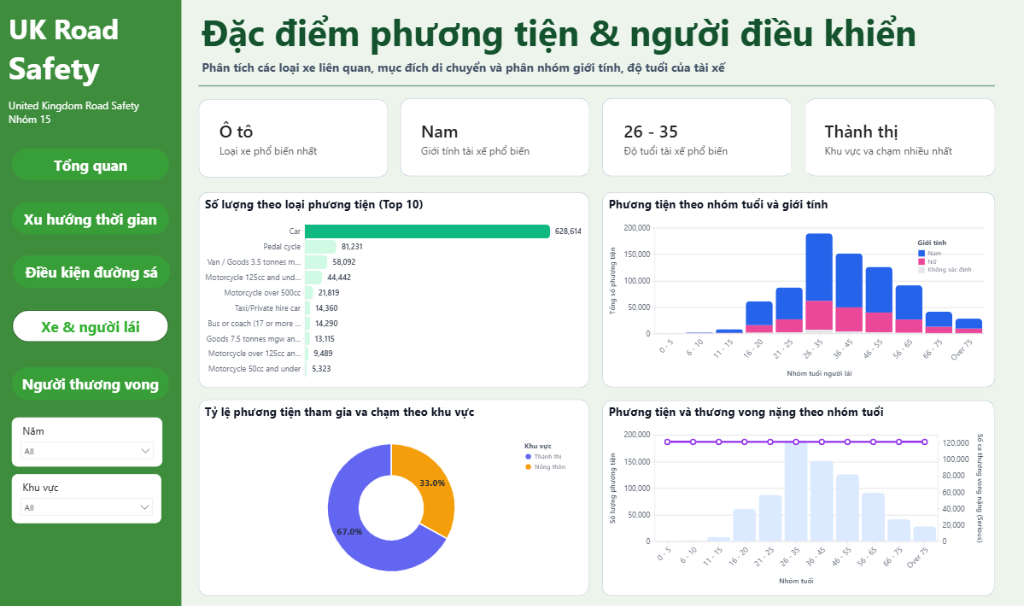
\includegraphics[width=\textwidth, keepaspectratio]{images/dashboard_page4.png}
        \caption{Phương tiện và người điều khiển}
        \label{fig:dashboard_page4}
    \end{subfigure}
    \hfill
    \begin{subfigure}[t]{0.48\textwidth}
        \centering
        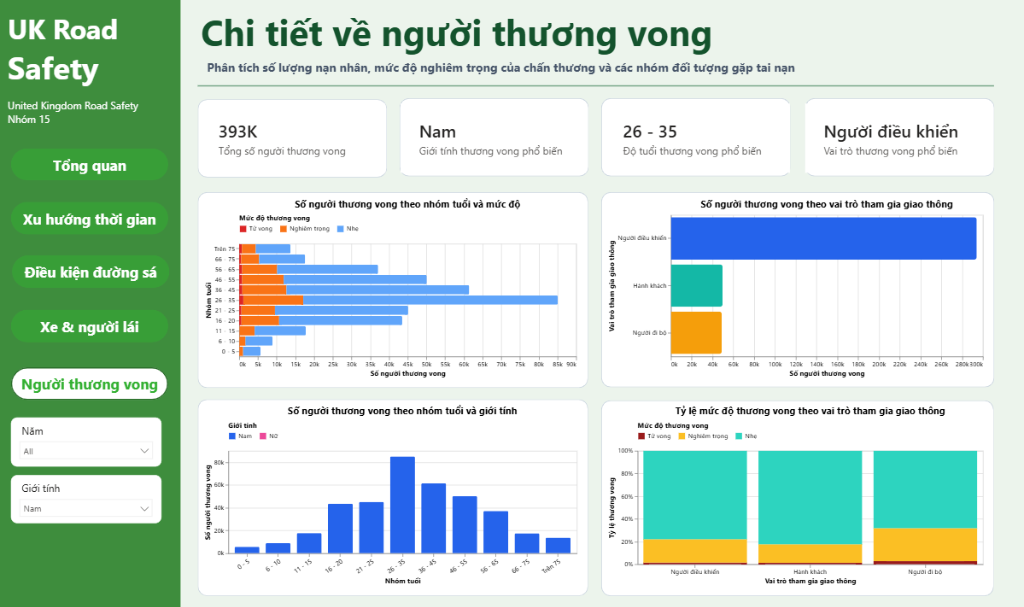
\includegraphics[width=\textwidth, keepaspectratio]{images/dashboard_page5.png}
        \caption{Người thương vong và nhóm rủi ro}
        \label{fig:dashboard_page5}
    \end{subfigure}
    \caption{Giao diện trang Phương tiện \& người điều khiển và Người thương vong}
    \label{fig:dashboard_group2}
\end{figure}

\textbf{Đặc điểm phương tiện và người điều khiển} (Hình~\ref{fig:dashboard_page4}) phân tích các khía cạnh liên quan tới phương tiện và tài xế. Thẻ KPI tổng hợp cho thấy loại phương tiện phổ biến nhất là Ô tô (Car), giới tính tài xế gặp nạn nhiều nhất là Nam, độ tuổi tài xế phổ biến nhất là từ 26--35 tuổi, và khu vực đô thị (Thành thị) chiếm tỷ trọng vượt trội (67%).

\textbf{Chi tiết về người thương vong và nhóm rủi ro} (Hình~\ref{fig:dashboard_page5}) tập trung sâu vào nạn nhân của các vụ tai nạn. Thẻ KPI thể hiện giới tính nạn nhân phổ biến là Nam, nhóm tuổi nạn nhân gặp rủi ro cao nhất là 26--35 tuổi, và vai trò của người thương vong phổ biến nhất là Người điều khiển phương tiện (Driver or rider). Cổng slicer cho phép lọc động theo giới tính và năm để phục vụ phân tích drill-down.


\newpage

\section{Nhận xét và Kết luận}
\label{sec:conclusion}

Phần này dùng để tổng hợp toàn bộ các kết quả phân tích dữ liệu từ Dashboard, đề xuất các khuyến nghị mang tính thực tiễn và liệt kê danh mục tài liệu tham khảo.

\subsection{Tổng hợp các phát hiện quan trọng (Insights)}
\textit{[Hướng dẫn điền: Nhóm tự tổng hợp từ 3 đến 5 phát hiện nổi bật nhất thu được từ hệ thống Dashboard. Các insights này cần là sự kết hợp thông tin giữa các chương phân tích trước đó của các thành viên (ví dụ: xu hướng thời gian kết hợp với phân loại đối tượng để thấy danh mục nào đang đi xuống, hoặc tương quan hiệu suất kết hợp với phân khúc chủ thể...)].}

\subsection{Đề xuất khuyến nghị}
\textit{[Hướng dẫn điền: Dựa trên các phát hiện ở trên, đề xuất từ 3 đến 4 hành động thực tế có thể triển khai ngay. Các đề xuất này phải xuất phát trực tiếp từ các con số hoặc xu hướng thực tế trong biểu đồ, tránh đưa ra các khuyến nghị mang tính chung chung không có căn cứ từ dữ liệu].}

\subsection{Kết luận đồ án}
Đồ án đã hoàn thành đầy đủ các nhiệm vụ và yêu cầu kỹ thuật do đề bài Lab 03 đặt ra. Thông qua việc tự tìm hiểu và thực hành trên môi trường Power BI Desktop kết hợp với sườn báo cáo LaTeX chuyên nghiệp, nhóm đã:
\begin{itemize}
    \item Tiếp cận và làm quen với quy trình phân tích dữ liệu chuyên nghiệp (chuẩn bị dữ liệu, làm sạch, liên kết mô hình, tính toán measure, trực quan hóa và khai phá tri thức).
    \item Xây dựng hệ thống Dashboard trực quan, thống nhất về mặt thẩm mỹ và có khả năng tương tác cao nhờ các bộ lọc slicers và tooltips động.
    \item Nâng cao năng lực làm việc nhóm thông qua phân chia nhiệm vụ rõ ràng và ráp nối các thành phần báo cáo khoa học.
\end{itemize}

---

\section{Tài liệu tham khảo}
\label{sec:references}

Dưới đây là danh sách các nguồn dữ liệu, tài liệu lý thuyết và trang web được sử dụng trong quá trình thực hiện đồ án:

\begin{enumerate}
    \item \textbf{Nguồn dữ liệu}: 
    \begin{itemize}
        \item Nguồn tải bộ dữ liệu chính: \textit{[Nhóm điền tên bộ dữ liệu và dán link liên kết công khai vào đây]}.
    \end{itemize}
    
    \item \textbf{Tài liệu về Power BI}:
    \begin{itemize}
        \item Microsoft Power BI Guidance: \url{https://learn.microsoft.com/en-us/power-bi/}
        \item Các tài liệu, bài giảng môn học Trực quan hóa dữ liệu từ Giảng viên.
    \end{itemize}

    \item \textbf{Tài liệu khác}:
    \begin{itemize}
        \item Tài liệu Overleaf Learn LaTeX: \url{https://www.overleaf.com/learn}
        \item \textit{[Thêm các tài liệu nghiên cứu liên quan đến chủ đề đề tài của nhóm nếu có...]}.
    \end{itemize}
\end{enumerate}


\end{document}
